\newpage

\section{Existujúce riešenia}

Počas analýzi som našiel niekoľko riešení problému dynamického odporúčania.
Každé z týchto riešení poskytuje rôzne výhody a nevýhody pri rôznych oblastiach
nasadenia. To ktorý model je najvhodnejší pre nás je ovplivnené cieľovím artiklom
a cieľovou skupinou. Pre potreby tejto práce bolo potrebné najskôr vybrať doménu,
v ktorej chcem riešenie implementovať. Následne zanalizováť prístupy v danej oblasti.

\subsection{Odporúčanie hudobných dokumentov}

Pre potreby tejto práce som zvolil oblasť hudby, avšak nie v úplne klasickom ponímani,
zameral som sa na dokumenty umožňujúce hudobníkom naučiť sa hrať určité hudobné dielo.
Za základne vlastnosti hudby sa považuje rytmus, sila a farba tónu.
Na zaznamenanie týchto vlastnosti vzniklo viacero zápisov podľa potrieb
určitých skupín hudobníkov. Odporúčanie v tejto oblasti je pomerne nové 
a preto sa budem skôr snažiť najsť riešenia z iných oblastí a preskúmať
ich aplikovateľnosť v tejto oblasti.

Na presné odporúčanie akého koľvek artiklu, musíme najskôr najsť nejaké jeho
vlastnosti na základe ktorý môžeme odporúčať. Keďže táto doména je úzko spojená z hudbov,
budem sa snažiť vychádzať z nej.

Najznámejším spôsobom kategorizovania hudby je rozdelenie na žánre a podžánre.
Problém pri žánroch a podžánroch je, že neexistuje jednotá definícia ani spôsob
ich kategorizácie. Určovanie zánrov ma nasledujúce typy pravidiel

\begin{itemize}
\item{\textbf{formálne a technické pravidlá aplikované na obsah(sila, výška a farba tónu)},}
\item{\textbf{semiotické pravidla} (abstraktný vopred dohodnuty koncept,
    napríklad politická situácia),}
\item{\textbf{pravidla správania sa} 
    (črty správania sa fanúčikov alebo interpretov daného žánru),}
\item{\textbf{ekonomické a jurisdikčné pravidlá} 
    (zákonné a právne aspekty ktoré daný žáner podporujú,
        napríklad český protestsong\footnote[1]{www.wikipedia.sk}).}
\end{itemize}

Tieto pravidlá definoval Franco Fabbri\cite{music_genres_problematics}.

Pravidlá sú pomerne abstraktné a i napríek viacerím pokusom o vytvorenie
kompletne ontológie žánrov či už z akademický alebo komerčných kruhov
\footnote[2]{https://www.apple.com/itunes/affiliates/resources/documentation/genre-mapping.html},
neexistuej jenotná ontológia hudobných žánrov.

Pre potrebý odporúčania by bolo najvhodnejšie automatické určovanie žánru, ako napríklad 
navrhli autory článku \cite{automatic_genre_recognition}, kde analizovali výšku
a snažíli sa odhaliť akcent nôt, čo im umožnilo odhaliť rymtus piesne. Následne sa zamerali
na určenie jednotlivých časti hudobného diela ako predohra, hlavná časť, refrén a sloha.

Ďaľším prístupom je nechať označovať vlastnosti dokumentu používateľom, tento prístup
používa napríklad služba last.fm\footnote[3]{http://www.last.fm/home}, ktorá sa následne
snaží používa najpopulárnejšie značky ako žánre. Tento prístup je bližšie opísany v článku 
Paual Lamera\cite{social_tagging_music} a je známy pod názvom socialne značenie 
(angl. social tagging).

\paragraph{Podobnosť odporúčania hudobných dokumentov a hudby}

I keď sú tieto dve domény veľmi podobné, existujú rozdiely. Jeden z rozdielov sú ich vlastnosti 
dokumentov. Na presnú identifikáciu pesníčky nám stačí názov piesne, autor piesne, interpret a 
prevedenie. Pri hudobných dokumentoch sa môžu okrem týchto vlastnosti líšiť aj v type dokuemntov
(taby, akordy, text, preklad), prípadne niektoré dokumenty môžu obsahovať iba časť daného
hudobného diela (predohra, medzi-hra, refrén, sólo atď.).

\paragraph{Podobnosť z odporúčaním textu}

Ďaľšia doména ktorú je možné využiť je odporúčanie textových dokumentov. To je najčastejšie 
založené na anlíze výskytu slóv v texte. Avšak jediné typy dokumentov ktoré by sa 
dali takto analizovať sú preklady a texty.

\subsection{Rôzne prístupy k odporúčaniu}

Hlavný účelom odporúčacích systémov je odhadnúť užitočnosť dokumentu pre
používateľa\cite{recommender_categories}, pričom v mnohých prípadoch
je potrebné užitočnosť dokumentu odhadovať. Užitočnosť ako taká môže závisieť od
veľkého množstva parametrov, skopina týhto parametrov sa všeobence nazýva
kontextové premenné. Na základe toho ako systém nakladá z danými údajmy, 
delím odporúčacie systémy na niekoľko kategórií. Hlavnou charakteristikov systému
je \textbf{funkcia užitočnosti}.

\paragraph{Filtrovanie na základe obsahu}

Pri tomto prístupe odporúčame používateľovy dokumenty podobné tým čo sa mu páčili
v minulosti. Funkciou užitočnosti dokumentu je teda podobnosť dokumentu z už zobrazenými
dokumentmi používateľa. Podobnosť dokumentov sa zisťuje pomocov porovnávania značiek dokumentov.

\paragraph{Kolaboratívne filtrovanie}

Toto je najpopulárnejší spôsob implementácie odporúčania. Najjednoduchšia a originálna 
implementácia odporúča aktívnemu používateľovy dokumenty ktoré sa páčili ľuďom z podobným
vkusom. Podobnosť používateľov je založená na historí hodnotenia dokumentov používateľov.
Takže úlohou funkcie užitočnosti je najsť najpodobnejších používateľov a vrátiť 
dokument ktorý mal najkladnejšie hodnotenia od týchto používateľov.

Najväčším problémom kolaboratívneho filtrovania, tzv. problém studeného štartu. Spočíva v tom
že ak pribudne do zbierky nový dokument, nemá ešte žiadne hodnotenia, takže sa nebude nikomu
odporúčať.

\paragraph{Demograficke odporúčanie}

Tieto odporúčacé systémi odporúčajú používateľovy dokumenty na základe jeho demografického
profilu (vek, národnosť, jazyk atď.). Za istú fomru tohoto odporúčania môžeme považovať
multijazičnosť dnešných stránok. Zaujímavým príkladom je aj domovska stránka google,
ktorá sa vo významné dni zobrazuje v rôznych krajinách
rôzne\footnote{http://www.google.com/doodles/}.

\paragraph{Znalostne odporúčanie}

Zanlostné odporúčacie systémy odporúčajú na základe znalostí o tom ako nejaká vlastnosť 
dokumentu ovplivňuje užitočnosť dokumentu pre používateľa. V princípe ide o systém
ktorý dáva používateľovy otázky a na základe zistených faktov mu odporučí dokument.
Takéto odporúčanie sa najčastejšie využíva pri zákazníckej podpore, 
veľmi dobrým príkladom na tento prístup je zákaznícka podpora
Microsoftu\footnote{https://support.microsoft.com/sk-sk}.

\paragraph{Komunitné odporúčanie}

Toto odporúčanie ja veľmi podobné s kolaboratívným filtrovaním, avšak na rozdiel od neho
upradnostňuje implicitne dané priateľstvá medzi používateľmi.  Tento druh odporúčania
zažíva rozkvet nejmä v poslednej dobe spolu z rozkvetom používania socialnych sieti.
V dokumente\cite{recommender_categories} sa dokonca uvádza že v špecialnych 
prípadoch sú efektívnejšie ako kolaboratívne filtrovanie.
Tento druh odporúčania sa často nazýva aj sociálne odporúčanie.
Funkcia užitočnosti v tomto prípade najskôr zistí vzťahy medzi používateľmy a 
preferencie priateľov používateľa a na základe ich preferencií určí užitočnosť dokumentov
pre používateľa.

\paragraph{Hybridné odporúčanie}

Toto odporúčanie kombinujé vlastnosti predchádzajúcich prístupov na vyriešenie ich vázjomných
problémov. Napríklad časté riešenie je kombinovanie colaboratívneho filtrovania z 
filtrovaním založeným na obsahu, kedy v podstate filtrovanie na základe obsahu rieši problém
studeného štartu pre kolaboratívne filtrovanie. Tak isto sa v poslednej dobe 
zvikne kombinovať kolaboratívne filtrovanie z komunitným odporúčaním
vďaka ich dobrým výsledkom.

\paragraph{Spätná vezba}

Aby odporúčacie systémy mali ako odporúčať, potrebujú zistiť preferované vlastnosti dokumentov
zo korpusu odporúčaných dokumentov. Z tohot dôvodu je potrebné nejakým spôsobom zistiť 
ktoré vlastnosti používateľ preferuje. Na toto zisťovanie slúži spätná väzba. 
Spätnú väzbu v zásade delíme na dve skupiny, 

\begin{itemize}
\item{\textbf{implicitná spätná väzba} (je získavanie spätnej väzby používateľa z jeho akcií
ktoré nesúvysia priamo z hodnotením, napríklad stiahnutie dokumentu, prípadne jeho vytlačenie, 
hlavnou výhodou je že nevyžaduje vedomí zásah používateľa, avšak zvyšuje technycké nároky na 
systém) }
\item{\textbf{explicitná spätná väzba} (je vedome ponúknutie spätnej väzby od používateľa,
napríklad ak používateľ označí že sa mu dokument páči, podľa \cite{basic_user_profiles}
zvykne byť efektívnejšia, avšak vyžaduje vedomy zásah používateľa )}.
\end{itemize}

Explicitnú spätnu väzbu môžeme ďalej deliť na základe toho, akú hodnotu nám vracia napríklad 
na \textbf{binárnu}, \uv{páči sa my} a \uv{nepáči sa mi}, alebo \textbf{z hodnotu} (napríklad
pridelovanie 1 až 5 hviezdičiek). S týmto priamo súvysí aj konštrukcia používateľských profilov.

\subsection{Používateľské profily}

Ďaľšou dôležitou súčasťou odporúčacích systémov je spôsob akým konštruujú používateľské profili.
Rôzne druhy profilov umožňujú použítie rôznych algoritmov avšak môžu mať rôzny dopad na 
pamäťovú či výkonovú stránku systému\cite{basic_user_profiles}.

\paragraph{Binárny vektor}

V tomto prípade sú preferencie reprezentované vektorom v dvojrozmernom priestore kde
jeden rozmer sú značky dokumentov a druhý sú používatelia. Vektor
je tvorený binárnou hednotou kde 1 na pozícií \(p_{ij}\), pri predpoklade že \(j\) je 
identifikátor \(j\).-teho používateľa a \(i\) je identifikátor \(i\)-tej značky,
znamená že \(i\)-ta značka je preferencia používateľa \(j\).
V tabuľke \ref{table:binaryprofile} môžeme vidieť príklad v ktorom máme používateľa \(p_0\)
ktorý nepreferuje žiadné značky, následne Používateľa \(p_1\) ktorý preferuje značky \(z_1\),
\(z_2\)
a Používateľa \(p_2\) ktorý preferuje značku \(z_0\).

\begin{table}[h]
\begin{center}
\begin{tabular}{|l|l|l|l|}
\hline
 \(z_p\) & \(p_0\) & \(p_1\) & \(p_2\) \\ \hline
\(z_0\) & 0     & 0        & 1        \\ \hline
\(z_1\) & 0     & 1        & 0        \\ \hline
\(z_2\) & 0     & 1        & 0        \\ \hline
\end{tabular}
\end{center}
\caption{Ukážka modelu profilu ako binárneho vektora}
\label{table:binaryprofile}
\end{table}

\paragraph{Vahovaný vektor}

Tento profil je veľmy podobný z predchádzajúcim profilom, avšak namiesto bynarných 
hodnôt sú hodnotamy súradníc užitočnosti daných preferencií \ref{table:weightprofile}.

\begin{table}[h]
\begin{center}
\begin{tabular}{|l|l|l|l|}
\hline
\(z_p\)  & \(p_0\) & \(p_1\) & \(p_2\) \\ \hline
\(z_0\) & 0     & 0        & 2        \\ \hline
\(z_1\) & 0     & 2        & 0        \\ \hline
\(z_2\) & 0     & 5        & 1        \\ \hline
\end{tabular}
\end{center}
\caption{Ukážka modelu profilu ako váhovaného vektora.}
\label{table:weightprofile}
\end{table}

\paragraph{Trojrozmenrý vektor}

V prípade že vieme aj rozdeliť značky do domén alebo kontextov,
môžeme do vektorového profilu pridať ešte jednú súradnicu ktorá reprezentuje
doménu dnej značky. Napríklad ak odporúčame text a značky sú
reprezentované slovamy ktoré sa našli v texte, tak značke ktorá pochádza 
z nadpisu môžeme automaticky priradiť väčšiu hodnotu.

\paragraph{Profil sémantickej siete}

Profil sémantickej siete (angl. Semantic network profile) je semantická sieť
ktorá je vybudovaná pre konkrétneho používateľa a vyjadruje vzťahy medzi značkamy
ktoré používateľ preferuje.


Sémantická sieť\cite{semantic_networks} je orientovaný graf v ktorom sú vrcholmi značky,
zatiaľ čo hrany sú ich vzťahy.
napríklad v \cite{basic_user_profiles} sú použité vzťahy typov.

\begin{itemize}
\item{konjunkcia,}
\item{disjunkcia,}
\item{substitúcia,}
\item{negácia.}
\end{itemize}

Takéto semantické siete sa používajú najmä pri dopĺňaní slov do vyhľadávacích fráz,
kde v prípade krátkej vyhľadávacej frázy môžeme zredkuvať jej viacznačnosť doplnením
slóv ktoré majú v sémantickej sieti najsilnejšiu pozitívnu väzbu.
Na obrázku \ref{fig:semantic_network} môžeme vidieť príklad takejto siete.

Teda ak by mi prišiel od používateľa výraz \textit{folk}, tak môžem výraz rozšíriť slovamy
\textit{akustika} a \textit{text}. Keď budem pokračovať, slovo text sa dá nahradiť slovom
akordy (keďže v podstate akordy sú text doplnení o skratky akordov). Následne však taby už
nemôžem doplniť aj keď majú disjunktný vzťah z akordamy, pretože majú silnú negativnú 
väzbu z folkom. Teda výsledný výraz by bol \textit{folk a akustika akordy}.

\begin{figure}
    \begin{center}
        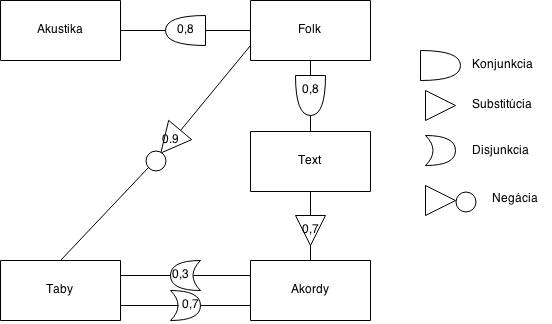
\includegraphics[scale=0.55]{semantic_network}
        \caption{Ukážka sémantickej siete}
        \label{fig:semantic_network}
    \end{center}
\end{figure}

\paragraph{Bayesova sieť}

Ďaľšou možnosťou ako ukladať používateľské dáta je bayesová sieť. Bayesová sieť vychádza z 
bajesovej teorémy, o ktorej využití v kontexte odporúčania sa budeme zaoberať neskôr.
Bayesová sieť slúži na výpočet pravdepodobnosti hypotézy pri zmene jej evidencie.
Jej vrcholmy sú latentné premenné (závisia od ostatných premenných) a jej hranamy ich vzťahy.
Takže v pípade že sa mi zmení hodnota jednej premennej v grafe, po hranách viem upraviť hodnoty 
všetkých premenných ktoré od nej závysia.

Napríklad na obrázku \ref{fig:bayes_network} môžeme vydieť bayesovú sieť zloženú z troch 
premenných \(a\), \(b\) a \(c\). Tieto sú vo vzájomnom vzťahu. V prípade zmený hodnoty \(a\)
alebo \(b\) sa hodnota \(c\) automaticky prepočíta.

\begin{figure}
    \begin{center}
        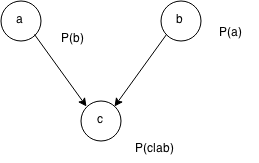
\includegraphics[scale=0.55]{bayes_network}
        \caption{Ukážka bayesovej siete}
        \label{fig:bayes_network}
    \end{center}
\end{figure}

Ako príklad ako využiť takúto sieť môžem uviesť zjednodušený príklad z
prezentácie \cite{probability_ir}, kde najhornejšie vrcholy (tie ktoré nezávyseli od iných 
premenných) boli dokumenty \(D = {d_1, d_2 ... d_n}\) a pod nimy
boli ich značky \(Z = {z_1, z_2... d_n}\), následne ak sme chcely odporúčať (príklad je 
aplikovaný na vyhľadávací dotaz, avšak dotaz môže byť nahradení používateľským profilom),
na najspodnejšie body sme pripojili preferencie používateľa \(P = {p_1, p_2... p_n}\).
Náčrt siete môžeme vydieť na obrázku \ref{fig:recommend_bayes_network}.

\begin{figure}
    \begin{center}
        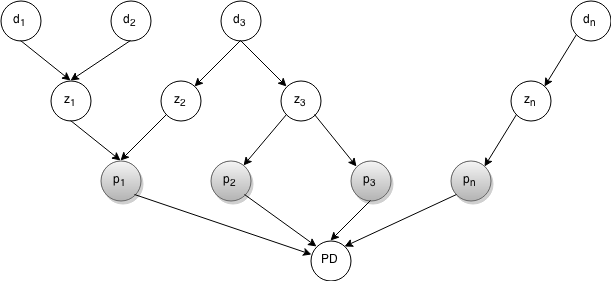
\includegraphics[scale=0.55]{recommend_bayes_network}
        \caption{Ukážka odporúčacej bayesovej siete}
        \label{fig:recommend_bayes_network}
    \end{center}
\end{figure}

Pričom značky a dokumenty si môžem držať predpočítané v pamäti, a tak isto aj používateľské 
preferencie. V prípade odporúčania ich iba poprepájam.

\paragraph{Bayesov theorem}

Bayesová teoréma sa zaoberá vyplivom nových poznatkov na existujúce 
domienky o určitej hypotéze. Vďaka nej vieme kombinovať nové dáta z existujúcimy poznatkami.
Matematicky je táto teoréma vyjadrená v kontexte vyhľadávania 
pomocov rovnice \ref{eq:bayes_theorem_rel} a rovnice \ref{eq:bayes_theorem_norel}.

\begin{equation} \label{eq:bayes_theorem_rel}
P(P|d) = \frac{P(d|P) * P(P)}{P(d)}
\end{equation}

\begin{equation} \label{eq:bayes_theorem_norel}
P(NP|d) = \frac{P(d|NP) * P(NP)}{P(d)}
\end{equation}

Rovnice obsahujú,
\begin{itemize}
\item{pravdepodobnosť že dokument je užitočný \(P\),}
\item{prevdepodobonsť že dokuemnt nie je užitočný \(NP\),}
\item{pravdepodobnosť že vrátený dokument \(d\) je užitočný \(P(P|d)\),}
\item{\(P(d|P)\) prevdepodobnosť že ak je vrátený užitočný dokument, je to dokument \(d\),}
\item{pravdepodobnosť vrátenia užitočného dokumentu \(P(P)\),}
\item{pravdepodobnosť výberu dokumentu \(P(d)\),}
\item{pravdepodobnosť neužitočnosti dokumentu \(P(NP|d)\),}
\item{pravdepodobnosť \(P(d|NP)\) že ak je ak je vrátený neužitočný dokument,
    je to dokument \(d\),}
\item{\(P(NP)\) je pravdepodobnosť že je vrátený neužitočný dokument,}
\item{pravdepodobnosť \(P(d)\) vrátenia dokumentu \(d\).}
\end{itemize}

To či je dokumentu užitočný sa následne určuje tým, či je \(P(P|d)\) väčšie ako \(P(NP|d)\).

\subsection{Váhovanie značiek}

Ak mám dokument alebo profil reprezentovaný značkamy, je potrebné zistiť ako veľmi sú tieto 
značky prefereované. Nie včetky značky majú rovnakú váhu, takže potrebujeme dosiahnuť 
aby užitočnosť dokumentu závisela od unikátnosti značiek v ňom. Základy váhovania sú popísané 
v prezentácií Hinrich Sch¨utze \cite{vector_space_model}.

\paragraph{Frequencia pojmov}

Frequencia pojmov (angl. Term Frequency ďalej TF),
je jeden z najjednoduchších a najstarších prístupov k váhovaniu značiek,
pri tomto prístupe sa jednoducho počíta počet výskytov značiek v dokumente.
Existuje niekoľko druhov tohoto váhovania.

\textbf{Binárne váhovanie} znamená že napríklad, nepočítam počet výskytov
slova v texte ale beriem iba či sa v texte nachádza alebo nie. Matematicky
vyjadrené rovnicou \ref{eg:binary_tf}.

\begin{equation} \label{eq:binary_tf}
    w_{TF_BIN}(t_i) = 
    \left\{
        \begin{array}{11}
            1   & \mbox{ak } t_i \in d_j \\
            0   & \mbox{ak } t_i \notin d_j
        \end{array}
    \right.
\end{equation}

Kde \(d_j\) je dokument a \(t_i\) je slovo.

\textbf{Čistá frequencia} sa dá tiež použiť, v tomto prípade sa
váha slova určuje podľa počtu jeho výskytov v texte. 
Matematicky vyjadrené rovnicou \ref{eq:count_tf}

\begin{equation} \label{eq:count_tf}
w_{TF_RAW}(t_i) = t_{i_{d_j}}
\end{equation}

Kde \(t_{i_{d_j}}\) je počet výskytov slova \(t_i\) v dokumente \(d_j\).

\textbf{Logaritmická váha} sa taktiež používa najmä kôly tomu, 
že relevancia dokumentu nerastie proporcionalne z počtom výskytov slova
v dokumente. Toto môžem matematicky vyjadriť napríklad rovnicou \ref{eg:log_tg}.

\begin{equation} \label{eq:log_tf}
    w_{TF_LOG}(t_i) = 
    \left\{
        \begin{array}{11}
            1 + \log{10}t_{i_{d_j}} \mbox{ak } t_{i_{d_j}} > 0 \\
            0 & \mbox{inak}
        \end{array}
    \right.
\end{equation}

Existuje ešte viac spôsobov ako sa dá vyhodnotiť frequencia pojmov, medzi ktoré patrí napríklad
dvojita normalizácia 0.5 (angl. double normalization 0.5) alebo
k-dvojita normalizácia (angl. double normalization K) \cite{vector_space_model}.

\paragraph{Frequencie pojmov, inverzna frequencia dokumentov}

Frequencia pojmov, inverzná frequencia pojmov 
(angl. Term Frequency, Inverse Document Frequency ďalej TF*IDF)
je prístup, pri ktorom zahrňujeme do užitočnosti aj počet dokumentov, ktoré majú danú značku.
Základom je zníženie užitočnosti často sa vyskytujúcim značkám.
Toto znižovanie je reprezentované rovnicou \ref{eq:idf} ďalej IDF.

\begin{equation} \label{eq:idf}
idf_i = log{10}\frac{N}{dt_i}
\end{equation}

Kde \(dt_i\) je počet dokumentov v ktorých sa pojem \(t_i\) nacháza.

Výsledna rovnica TF*IDF je rovnica \ref{eq:tfidf} ktorá je vlastne súčin TF a IDF.

\begin{equation} \label{eq:tfidf}
w_{TF*IDF} = w_{TF} * log{10}\frac{N}{dt_i}
\end{equation}


\paragraph{Presonalizované BM25 váhovanie}

Tento model je jeden zo štatystických modelov. Tu uvedená verzia je 
jeho modifikácia podľa S. Cronen a spol. \cite{modified_bm25} ktorá
je matematický reprezentovaná rovnicou \ref{eq:bm25}.

\begin{equation} \label{eq:bm25}
w_{BM25}(t_i) = \log{
    \frac{(r_{t_i} + 0.5)(N - n_{t_i} + 0.5)}
        {(n_{t_i} + 0.5)(R - r_{t_i} + 0.5)}}
\end{equation}

Kde \(N\) je počet všetkých dokumentov, \(n_{t_i}\) je počet
dokumentov obsahujúcich pojem \(t_i\), R je počet dokumentov
ktoré používateľ už navštívil a \(r_{t_i}\) je počet dokumentov ktoré
už používateľ navštíciľ obsahujúcich pojem \(t_i\)

\subsection{Evolúcia používateľských preferencií}

Preferencie používateľa sa z časom menia, môžu vznikať nové a zanikať staré,
prípadne sa vracať predošlé. Na základe toho môžeme používateľské preferencie rozdeliť
na 

\begin{itemize}
\item{krátkodobé preferencie,}
\item{dlhodobé preferencie,}
\item{sezónne preferencie.}
\end{itemize}

Odhalenie krátkodobých záujmov je pomerne trivialne, stačí agregovať používateľové záujmi
za časové obdobie ktoré považujeme za \uv{krátku dobu} a vrátiť značky ktoré používateľ 
preferoval najčastejšie.

\paragraph{Dlhodobé záujmy}

Problém dlhodobých záujmov je o dosť komplikovanejší, väčšina riešení ktoré som preskúmal
používala na tento problém kombináciu rôznych váhovacích algoritmov a štatystických metód.
Napríklad v článku \cite{long_term_profile}, kde použíli už spomínané váhovacie 
algoritmy.

Používateľský profil je reprezentovaný trojrozmerný váhovaným vektorovým profilom
a zoznamom zobrazených dokumentov (navštívené url).
Následne sa najskôr vytvorí zoznam adekvátnych dokumentov zo
značiek. Následne na porovnávanie značiek dokumentov a profilov sa používajú tri rôzne
algoritmy.

\textbf{Jednoduché porovnávanie} kde sa vlastne spočítajú váhy značiek ktoré 
majú spoločné používateľ a dokument podľa vzorca \ref{eq:matching}.

\begin{equation} \label{eq:matching}
u_{j}(d_i) = \sum\limit_{t=1}^N_{z_t}f(z_t) * u(z_t)
\end{equation}

Vysledkom je funkcia užitočnosti pre dokument i \(u_{j}(d_i)\), \(N_{z_i}\) je počet unikátnych
značiek v dokumente \(d_i\), \(f(z_t)\) je počet výskytvo značky \(z_t\) v dokumente a
\(u(z_t)\) je vypočítaná užitočnosť značky \(z_t\).

\textbf{Porovnávanie unikátnych} značiek, teda zanedbávame váhu určenú váhovacími algoritmamy a
iba spočítame unikátne značky podľa vzorca \ref{eq:unique_matching}.

\begin{equation} \label{eq:matching}
u_{u}(d_i) = \sum\limit_{t=1}^N_{z_i} u(z_t)
\end{equation}

\textbf{Jazykový model} (angl. Language model) ktorý generuje unigramovy jazykovy model
(angl. unigram language model) kde užitočnosť značiek je použitá ako ako frekvencia značiek
v rovnicy \ref{eq:language_model}.

\begin{equation}\label{eq:language_model}
u_{lm}(d_i) = \sum\limit_{t=1}^N_{z_i}\log{\fract{u(z_t) + 1}{\sum\limit_{j=1}^N_{z_i}}}
\end{equation}

Ďalej sa ešte výsledne dokumenty poskytnuté jednym z týchto algoritmov ešte filtruju algoritmom
PClick, ktorý pracuje z históriou navštívených dokumentov. Tento algoritmus vracia iba dokumenty
ktoré používateľ v histó často navštevoval. Matematický je to vyjadrené rovnicou \ref{eq:pclick}.
Tento algoritmus berie do úvahy aj vyhľadávacií dotaz.


\begin{equation} \label{eq:pclick}
u_{pclick}(d_i) = \frac{|Zobrazenia(d_i, u_j, q_n)|}{|Zobrazenia(q_n, u_j)| + \beta}
\end{equation}

Kde \(Zobrazenia(d_i, u_j, q_n)\) je počet zobrazení dokumentu \(d_i\) a 
\(Zobrazenia(q_n, u_j)\) je celkový počet zobrazení dokumentu \(d_i\)
pre vyhľadávací dotaz \(q_i\).

Ďaľším možné riešenie som našiel v článku Ferida Achemoukh a spol. \cite{achemoukh}. Toto
riešenie využíva hľavne štatystické metódy. Používateľa modeluje ako bayesovú sieť ktorú
modeluje pre niekoľko sedení ktoré sa skladajú z niekoľkých používateľových interakcií zo 
systémom.

% Ak málo regression model, exponentia decay, logovanie (dekstopova apka, webová, plugin 
% do chromu
